\documentclass[aps,pra, onecolumn,superscriptaddress,nopacs,floatfix, showkeys, notitlepage]{revtex4-1}
%   \documentclass[10pt]{article}



\usepackage{graphicx, color}
\usepackage{amssymb, amsmath}
\usepackage{times}
\usepackage[normalem]{ulem}
\usepackage{bbm}
\usepackage{todonotes}
\usepackage{mathtools}
\usepackage{enumitem} 
\usepackage{physics}
\usepackage{braket}
\usepackage{soul,xcolor}
\usepackage{subcaption}
\usepackage{bbold}
\usepackage{wrapfig}
\usepackage{multirow}

\usepackage{booktabs}  % for \toprule, \midrule, and \bottomrule macros 
\usepackage{tabularx}  % for 'tabularx' environment and 'X' column type
%\usepackage[hang,small,bf]{caption}
%\setlength{\captionmargin}{25pt}
%\usepackage{dblfloatfix}
\usepackage{tikz}
%%%<
\usepackage{verbatim}
%\usepackage[active,tightpage,floats]{preview}
%\PreviewEnvironment{tikzpicture}
%\setlength\PreviewBorder{5pt}%
%%%>
\usetikzlibrary{arrows}
\usetikzlibrary{positioning}
% Nice captions.
%\usepackage[hang,small,bf]{caption}
%\setlength{\captionmargin}{25pt}

% New commands to keep things tidy.
%\newcommand{\ket}[1]{$\left|#1\right\rangle$}
\newcommand{\Om}[1]{\small $\omega_{#1}$}
\newcommand{\De}[1]{$\Delta_{#1}$}
\newcommand{\Ga}[1]{$\Gamma_{#1}$}

%\newcommand{\Om}[1]{\small $\omega_{#1}$}
%\newcommand{\De}[1]{$\Delta_{#1}$}
%\newcommand{\Ga}[1]{$\Gamma_{#1}$}

\makeatletter
\newcommand*\bigcdot{\mathpalette\bigcdot@{.5}}
\newcommand*\bigcdot@[2]{\mathbin{\vcenter{\hbox{\scalebox{#2}{$\m@th#1\bullet$}}}}}
\newcommand*\cav{(\bigcdot)}
\newcommand*\ncav{(\bigcdot \bigcdot)}
\makeatother

%\newcommand{\ket}[1]{$\left|#1\right\rangle$}

\usepackage{amsmath}
\makeatletter
\def\env@cases{%
  \let\@ifnextchar\new@ifnextchar
  \left\lbrace
  \def\arraystretch{1.2}%
  \array{l@{\quad}l@{}}% Formerly @{}l@{\quad}l@{}
}



\begin{document}
\title{Note on 1D model of an FBG cavity and temperature sensitivity}
\author{NanoQT}
\date{\today}

\begin{abstract}
\textcolor{red}{}
\end{abstract}


\maketitle
%\tableofcontents



% \subsection{Fiber Bragg grating}
% The transmission of FBG mirror 
% \begin{figure}[!h]  
%         \centering
%         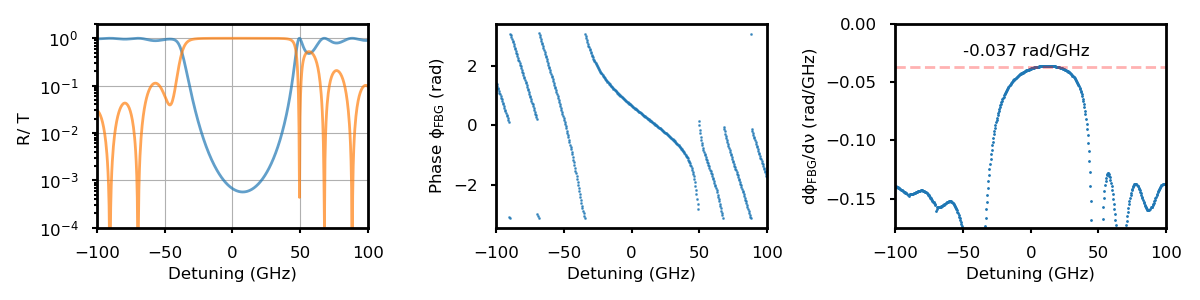
\includegraphics[width=1\linewidth]{fig/phase.png}
% 	\caption{Transmission/Reflection spectra and phase shift of a single FBG, estimated by a 1D model including the spatial inhomogenity of refractive index modulation $\delta n$. The inhomogenity is hand-picked by using a gaussian envelope with $\sigma=5$ mm and peak $\delta n = 3.6\times 10^{-4}$, leading to the asymmetry of the transmission/reflection spectra with respect to detuning (typically observed in the current system). The most right plot shows $\frac{\partial \phi_\mathrm{FBG}}{\partial}\sim-0.037$ rad/GHz at the mid gap
%  %and $\frac{\partial \phi_\mathrm{FBG}}{\partial}\sim-0.1$ rad/GHz near the bandedge.
%  }
%     \label{fig:1dsim}
% \end{figure}


%\section{Properties of a FBG cavity}
\section{1D model of an FBG cavity and approximate relations}
As described in the previous note \cite{note_temp}, the frequency response of an FBG is described by using a 1D model. 
Combined with the propagation of the distance $L_0$ between two FBGs, one can evaluate the properties of the FBG cavity, shown in Fig. \ref{fig:comp} (blue).
In the case of a high-finesse cavity, major cavity properties, including the external coupling rate $\kappa_\mathrm{ex}$, location of $m$-th cavity resonance $\nu_m$ and free-spectral range $\Delta_m$, are characterized by using the following approximate relations as 
\begin{eqnarray}
\kappa_\mathrm{ex}&\approx&\frac{1}{2}\Delta_0 \mathcal{T}_\mathrm{FBG}(m\cdot \Delta_0)\label{eq:kapp}\\
    \nu_m &\approx& \Delta_{0}\left(m-\frac{\phi_\mathrm{FBG}(m\cdot \Delta_{0})}{2\pi}\right)\label{eq:cav}\\
    \Delta_{m}&\approx &\Delta_{0}\left(1-\frac{1}{2\pi}\frac{\partial \phi_\mathrm{FBG}}{\partial \nu}\Delta_{0}\right),\quad\mathrm{where}\quad \Delta_{0}=\frac{c}{2n L_0}.
\end{eqnarray}
where transmittance $\mathcal{T}_\mathrm{FBG}(\nu)$ and phase shift of the FBG $\phi_\mathrm{FBG}(\nu)$, and a \textit{bare} free-spectral range $\Delta_0$.
\begin{figure}[!h]  
        \centering
        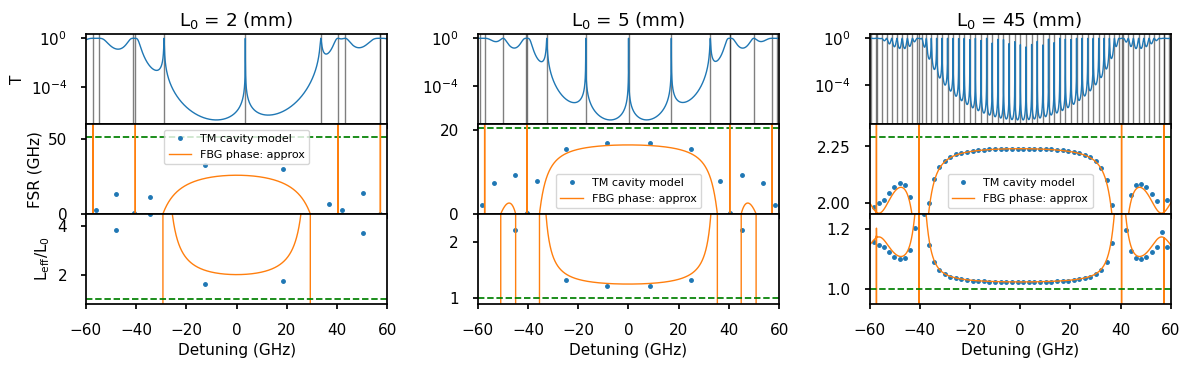
\includegraphics[width=1\linewidth]{fig/disperson.png}
	\caption{Comparison between 1D model of a FBG cavity (blue) and approximate relations (orange) for the transmittance (top), free-spectral range (middle) and effective cavity length $L_\mathrm{eff}$ over the physical distance between two FBGs $L_0$ (bottom). Note that $L_\mathrm{eff}$ is extracted from the inverse of the FSR.  (left) the length between two FBGs $L_0=2$ mm,  (middle) 5 mm, (right) 45 mm, similar to the current design.}
    \label{fig:comp}
\end{figure}
Note that $\mathcal{T}$ represents the transmittance while $T$ corresponds to the temperature in the following.


\section{Thermal tuning}
\subsection{Silica temperature dependence}
First, let us consider the temperature dependence of FBG and cavity length, made of silica. 
The resonance frequencies of the FBG $\nu_B$ and cavity mode $\nu_m$ can be written by using the unit cell length of FBG $\Lambda$ and cavity length $L$ (later discuss the heating effect of nanofiber and outside regions specifically)  as
\begin{eqnarray}
    \nu_B = 2 n \Lambda,\quad
    \nu_m = m\frac{c}{2n L},
\end{eqnarray}
Thus, the temperature dependence can be described by the thermo-refractive and elastic contributions since 
\begin{eqnarray}
    \frac{\partial \nu_B}{\partial T }&=& \nu_B\left(\frac{1}{n}\frac{\partial n}{\partial T}+\frac{1}{\Lambda}\frac{\partial \Lambda}{\partial T}\right) \approx  \nu_B\alpha_n\\
    \frac{\partial \nu_m}{\partial T }&=& -\nu_m\left(\frac{1}{n}\frac{\partial n}{\partial T}+\frac{1}{L}\frac{\partial L}{\partial T}\right)\approx -\nu_m\alpha_n.\label{eq:thermo-refractive}
\end{eqnarray}
In the last line, we use the fact that the thermorefractive coefficient $\alpha_n$ is dominant as
\begin{eqnarray}
    \alpha_n=\frac{1}{n}\frac{\partial n}{\partial T}=8\times 10^{-6}~\mathrm{(1/K)} \gg \alpha_L=\frac{1}{L}\frac{\partial L}{\partial T}=6\times 10^{-7}~\mathrm{(1/K)}.
\end{eqnarray}
Considering the small bandwidth of the stopband of FBG, $\sim 100$ GHz, compared to the resonant frequency, $\nu_B\sim 100$ THz, the range of cavity resonant frequency $\nu_m$ is small, leading to the relation of,
\begin{eqnarray}
    \frac{\partial \nu_B}{\partial T }\approx -\frac{\partial \nu_m}{\partial T } \approx \nu_B \cdot \alpha_n =3.1~\mathrm{GHz/K},\quad\mathrm{when~~\nu_B = 351.7~THz}
    \label{eq:nu_n}
\end{eqnarray}
We note that the temperature dependence of FSR can be safely ignored via
\begin{eqnarray}
    \frac{\partial \Delta_0}{\partial T }&\approx&-\Delta_0 \cdot\alpha_n \ll  \frac{\partial \nu_m}{\partial T }
    \label{eq:fsr_n}
\end{eqnarray}
due to the suppression ratio of $\Delta_0/\nu_B\lesssim 10^{-3}$.
%Here we only consider the thermorefractive index change, characterized by a thermo-refractive coefficient of silica $\alpha_n=\frac{1}{n}\frac{\partial n}{\partial T}=8.6\times 10^{-6}$ (1/K) at 300 K, since the thermo-elastic coefficient is one order-of-magnitude smaller.
In the following, we discuss the temperature sensitivity of external coupling rate $\kappa_\mathrm{ex}$ and cavity resonance frequency $\nu_m$.

\subsection{FBG mirror: external coupling rate}
%where the phase shift of FBG mirrors $\phi_\mathrm{FBG}$. 
Now, we can explicitly write down the temperature dependence of each parameter by using Eq. (\ref{eq:kapp}, \ref{eq:nu_n}, \ref{eq:fsr_n}) as
\begin{eqnarray}
%    \frac{\partial\nu_B }{\partial T }&=& \frac{\nu_B}{n}\frac{\partial n}{\partial T}= \nu_B\cdot\alpha_n= 3.06~\mathrm{GHz/K}, \quad \mathrm{where}\quad\nu_B=2n\Lambda\\
        \frac{\partial\kappa_\mathrm{ex} }{\partial T} 
        =\frac{1}{2}\left(\frac{\partial \Delta_0}{\partial T }\mathcal{T}_\mathrm{FBG}+\Delta_0 \frac{\partial \mathcal{T}_\mathrm{FBG}}{\partial T }\right)\approx\nu_B\cdot \alpha_n \cdot\left(\frac{\partial \kappa_\mathrm{ex}}{\partial \nu}\right).
%        \frac{\partial \nu_m}{\partial T}&\approx& \nu_B\cdot \alpha_n\cdot \left(\frac{\Delta_0}{2\pi}\frac{\partial \phi_\mathrm{FBG}}{\partial \nu}\right)
\end{eqnarray}
To illustrate the temperature dependence of the current device, we compute the FBG properties based on a 1D model using a transfer matrix method, as described in Ref. \cite{Bendickson1996} and Appendix \ref{app:1dmodel}.
Note that the simulation is done for the Cs parameters ($\nu_B=351.72$ THz), but a similar discussion is applicable to the telecomband case since the material properties are almost the same.
Figure \ref{fig:fbgtuningGaussian} shows the transmission spectra of a single FBG, $T_\mathrm{FBG}$, and the extracted temperature dependence of the external coupling rate, $\partial \kappa_\mathrm{ex}/\partial T$.
Although we consider a non-uniform refractive index modulation using the Gaussian envelope with $\sigma=L_\mathrm{FBG}$, the change of temperature dependence is small in the current parameter regime. 


%Add comparison of projected FSR and transfer matrix calculation.

\begin{figure}[!h]  
        \centering
        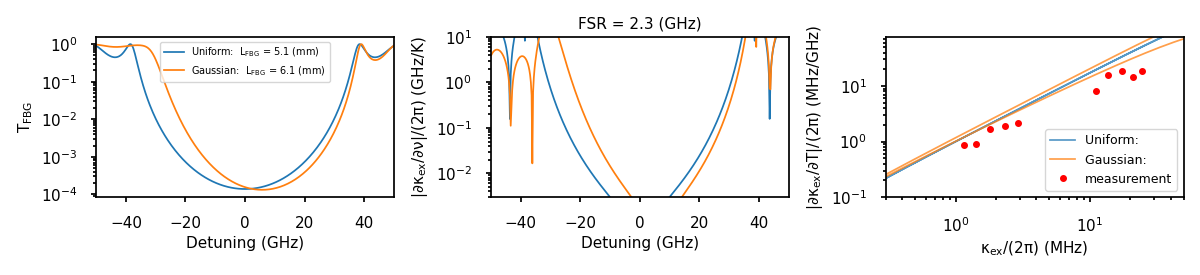
\includegraphics[width=1\linewidth]{fig/FBG_tuning_nonuni.png}
    	\caption{Temperature dependence of the external coupling rate $\kappa_\mathrm{ex}$. (left) Transmission of a single FBG; (blue) uniform refractive index modulation of $\delta_n=4.3\times 10^{-4}$ and FBG length of $L_\mathrm{FBG}=5.1$ mm. (Orange) gaussian distribution of refractive index modulation with $\sigma=5.9$ mm and peak $\delta n=4.3\times 10^{-4}$. The cavity length of 5.9 mm is chosen to match the similar minimum transmittance. (middle)\textcolor{red}{[typo: unit of y axis MHz/GHz]} Calculated $\left|\partial \kappa_\mathrm{ex}/\partial T\right|$ at $\Delta_0=2.3$ GHz. (right) \textcolor{red}{[typo: unit of y axis MHz/K]}Replotted to illustrate $\kappa_\mathrm{ex}$ dependence. The scaling of the measured data reasonably agrees with calculated scaling.}
    \label{fig:fbgtuningGaussian}
\end{figure}

\subsection{Cavity resonance frequency}
To consider the nanofiber heating separately \cite{note_temp}, we treat the nanofiber temperature $T_\mathrm{n}$ and the FBG temperature $T_\mathrm{f}$, separately. In addition, the cavity length $L_0$ is divided into two parts; \textit{nanofiber} regions and \textit{ other} with the optical length of $n_\mathrm{n} L_\mathrm{n}$ and $n_\mathrm{o} L_\mathrm{o}$, respectively. 

(i) The FBG temperature coefficient is given by using Eq. (\ref{eq:cav}) as
\begin{eqnarray}
        \frac{\partial \nu_m}{\partial T_\mathrm{f}}\approx \nu_B\cdot \alpha_n\cdot \left(\frac{\Delta_0}{2\pi}\frac{\partial \phi_\mathrm{FBG}}{\partial \nu}\right)
        \sim 487~\mathrm{MHz/K}\cdot \left(\frac{\Delta_0}{1~\mathrm{GHz}}\right)\cdot \left(\frac{\partial \phi_\mathrm{FBG}/\partial \nu}{1.0 ~\mathrm{rad/GHz}}\right)
\end{eqnarray}
where the slope of the phase $\phi_\mathrm{FBG}$ is shown in Fig. \ref{fig:fbgtuningGaussian}.
At the region of our interest, from the bottom of the stopband to the edge, this coefficient ranges $\frac{\partial \nu_m}{\partial T_\mathrm{f}}\sim 10-100$ MHz/K, resulting in the sufficiently large cavity frequency shift that needs to be stabilized by the nanofiber heating. 
\begin{figure}[!h]  
        \centering
        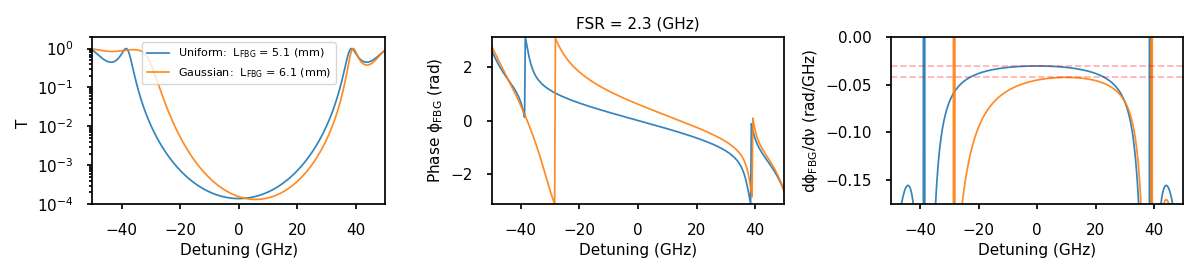
\includegraphics[width=1\linewidth]{fig/FBG_phase.png}
    	\caption{(left) Transmittance of a single FBG with uniform (blue) and gaussian distribution of $\delta n$ (orange). (middel) Phase of the single FBG. (right) The slope of $\phi_\mathrm{FBG}$ are given by $\partial \phi_\mathrm{FBG}/\partial \nu=-3.0\times 10^{-2}$, $-4.2\times 10^{-2}$ (rad/GHz), respectively.}
    \label{fig:fbgtuningGaussian}
\end{figure}


(ii) The nanofiber heating, localized at the nanofiber region of $L_\mathrm{n}$ due to the limited thermal conductactivity to the tapered regions, is simply given by,
\begin{eqnarray}
    \frac{\partial \nu_m}{\partial T_\mathrm{n}}=-\frac{n_\mathrm{n} L_\mathrm{n}}{n_\mathrm{n} L_\mathrm{n}+n_\mathrm{o} L_\mathrm{o}}\frac{\nu_m}{n_n}\frac{\partial n_n}{\partial T}\approx -\nu_B\cdot\alpha_n\cdot \eta,\quad \mathrm{where}\quad \eta=\frac{n_\mathrm{n} L_\mathrm{n}}{n_\mathrm{n} L_\mathrm{n}+n_\mathrm{o} L_\mathrm{o}}
\end{eqnarray}
where the ratio $\eta$ characterizes the average temperature over the entire cavity length.

Overall, the cavity frequency shift $\delta\nu_m$ is given by using the temperature change of FBG $\delta T_\mathrm{f}$ and nanofiber $\delta T_\mathrm{n}$ as
\begin{eqnarray}
    \delta\nu_m=\nu_B\cdot\alpha_n\left(\frac{\Delta_0}{2\pi}\frac{\partial \phi_\mathrm{FBG}}{\partial \nu}\delta T_\mathrm{f}-\eta\cdot\delta T_\mathrm{n}\right),\quad\mathrm{where}\quad \Delta_0=\frac{c}{2(n_nL_n+n_oL_o)}.
    \label{eq:cavshift}
\end{eqnarray}
 


\subsubsection{Frequency response}
\textbf{FBG thermal response:} Each FBG mirror is mounted on the Si-wafer using a vacuum compatible UV glue.
The Si wafer absorbs visible to near infrared light since the band gap of Si is 1.1 eV, corresponding to 1.1 $\mu$m.
The thermal conductivity of MACOR is sufficiently small and two FBGs are thermally isolated by the nanofiber region \cite{wuttke2013}, enabling us to control the FBG temperature independently by adjusting each laser power.
Due to the slow heat transfer from the Si wafer to the optical fiber with FBG, the $1/e$ time constant is tens of seconds.
Fig. \ref{fig:fdep} (left, bottom) shows the cavity frequency instability with the cavity locked to the Cs resonance using the thermal tuning of the FBG dispersion, suggesting a feedback timescale of a few tens of seconds.
This slow time scale could be improved by directly heating the fiber cladding (needs investigation).

\textbf{Nanofiber:} The nanofiber waist is heated by sending a guided-mode laser through the nanofiber. 
Since the fiber resides in an ultrahigh vacuum chamber and heat transport is dominated by far-field heat radiation \cite{wuttke2013}, the temperature at the nanofiber region ranges from room temperature up to and beyond 1000 K.
Figure \ref{fig:fdep} (right,top) shows the amplitude and phase of the response, showing the first-order pole with a corner frequency of $\sim$3 Hz. 
Considering the free-running stability of $\sim 1$ MHz/s, the tuning range is sufficient to remove the long-term drift of the cavity. 


\begin{figure}[!h]  
        \centering
        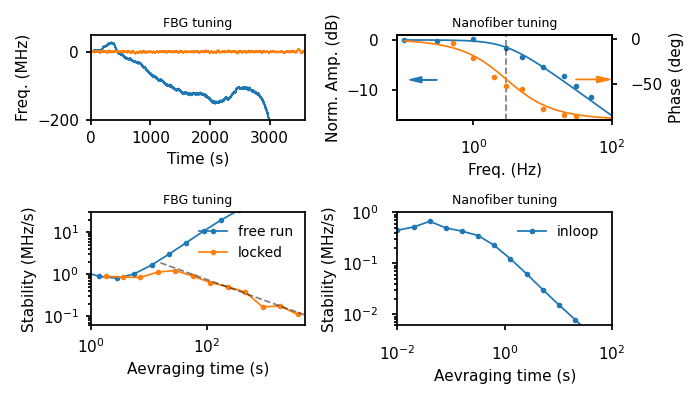
\includegraphics[width=0.6\linewidth]{fig/freq_response.png}
	\caption{Bandwidth of thermal tuning via FBG and nanofiber. (left, top) Time stamp of cavity frequency, locked to Cs transition via FBG dispersion tuning (orange) and free running (blue). (left, bottom) their stability, showing a few tens of seconds to acquire lock. (right, top) Transfer function of nanofiber heating with 3 Hz corner frequency. (right, bottom) a typical instability of the error signal.}
    \label{fig:fdep}
\end{figure}

\subsection{Cavity tuning using the Macor jig}
According to online specification sheets, the nanofiber holding jig, made of Macor, has a thermal expansion coefficient of $\alpha_j \approx 9\times10^{-6}$ per K.

\begin{eqnarray}
    \frac{dL}{dT_j} = \alpha_j L
\end{eqnarray}
Only considering the length variation of the jig, and assuming that the group velocity is uniform along the cavity, that the fiber pull against the thermal expansion of the jig can be neglected, and that the entirety of the cavity is extended uniformly, the resonance frequency dependence to jig temperature $T_j$ is given as
\begin{eqnarray}
\frac{d\nu_m}{dT_j}
= -\,\nu_m\,\alpha_j \approx -2~\mathrm{GHz/K}
\end{eqnarray}
at $\nu_m \approx 215~\mathrm{THz}$.

We note that if the jig temperature varies, the fiber temperature will also vary. Adding the two effects using eq.~\ref{eq:thermo-refractive}, we obtain about twice the result since $\alpha_j \sim \alpha_n$.
\begin{eqnarray}
\frac{d\nu_m}{dT}
= -\,\nu_m\,(\alpha_n + \alpha_j)\approx -4~\mathrm{GHz/K}
\end{eqnarray}

Let us reconsider the approximations. Silicon has a low thermal expansion ($\sim 2.5\times10^{-6} ~\mathrm{1/K}$ compared to Macor, so should not play a significant role. The Young's modulus of Macor and fused silica are similar(67~GPa and 72~GPa), and the effective cross section of the Macor is much larger, so that the fiber cannot pull back against the Macor. The glue could be a weak point, but for the 30 mm distance in question, we obtain $\Delta L \sim 300~\mathrm{nm}$ per K, which is negligible compared to the jog pulls of 10s of um.
However, the group velocity is not uniform and the cavity will not extend uniformly and the elasto-optic coefficient for fused silica could play a role, especially for the thinnest region. Need to estimate the effect.
% ============================================================
% 1. Non-uniform rod under axial extension
% ============================================================

\textbf{Non-uniform rod under axial extension}

Let a rod have length $L$ and a spatially varying cross section $A(x)$.
The material has Young's modulus $E$ and is pulled so that the total
extension is $\Delta L$.

The axial force is uniform along the rod:

\[
\sigma(x) = \frac{F}{A(x)}, \qquad
\varepsilon(x) = \frac{\sigma(x)}{E} = \frac{F}{E\,A(x)}.
\]

The total extension condition gives

\[
\Delta L = \int_0^L \varepsilon(x)\,dx
         = \frac{F}{E} \int_0^L \frac{1}{A(x)}\,dx.
\]

Define
\[
J = \int_0^L \frac{1}{A(x)}\,dx.
\]

Then the axial force is

\[
F = \frac{E\,\Delta L}{J}.
\]

The displacement distribution is

\[
u(x)
= \int_0^x \varepsilon(s)\,ds
= \Delta L\,
  \frac{\displaystyle \int_0^x \frac{1}{A(s)}\,ds}
       {\displaystyle \int_0^L \frac{1}{A(s)}\,ds}.
\]

Thus the local strain is

\[
\boxed{
\varepsilon(x)
= \Delta L\,
  \frac{\dfrac{1}{A(x)}}
       {\displaystyle \int_0^L \frac{1}{A(s)}\,ds}
}.
\]


% ============================================================
% 2. Local refractive-index change from axial strain
% ============================================================

\textbf{Local refractive-index change due to strain}

For an isotropic material (e.g. fused silica), axial strain causes
a local refractive-index change via the photoelastic effect:

\[
\Delta n(x) = -\,n\,p_e\,\varepsilon(x),
\]

where $n$ is the unstrained refractive index and $p_e$ is the effective
strain-optic coefficient (for silica, $p_e \approx 0.22$).

Combining with the strain distribution above, the local refractive-index
change is

\[
\boxed{
\Delta n(x)
= -\,n\,p_e\,\Delta L\,
  \frac{\dfrac{1}{A(x)}}
       {\displaystyle \int_0^L \frac{1}{A(s)}\,ds}
}.
\]

This shows that the refractive-index change is largest in the thinnest
regions of the rod (where $A(x)$ is smallest).

% ============================================
% Summary: OPL variation under nonuniform strain
% ============================================

% ==========================================
% OPL with effective index (short derivation)
% ==========================================

\textbf{Optical path length with effective index}

In the undeformed configuration $s \in [0,L_0]$,
\[
\mathrm{OPL}
= \int n_{\rm eff}(x)\,dx
= \int_0^{L_0} f(s)\,n_{\rm si}(\varepsilon(s))\,\bigl(1+\varepsilon(s)\bigr)\,ds.
\]

Expand $n_{\rm si}$ to first order in strain:
\[
n_{\rm si}(\varepsilon) = n_0 + n_\varepsilon\,\varepsilon,
\qquad
n_\varepsilon := \left.\frac{\partial n_{\rm si}}{\partial \varepsilon}\right|_{\varepsilon=0}.
\]

Insert into OPL and keep only first--order terms:
\[
\mathrm{OPL}
\simeq \int_0^{L_0}
f(s)\,\bigl[n_0 + n_\varepsilon \varepsilon(s)\bigr]\,(1+\varepsilon(s))\,ds
\]

\[
\simeq
\int_0^{L_0}
f(s)\,\bigl[n_0 + n_0\,\varepsilon(s) + n_\varepsilon\,\varepsilon(s)\bigr]\,ds.
\]

Thus:

- Unstrained optical path length:
\[
\mathrm{OPL}_0 = \int_0^{L_0} f(s)\,n_0\,ds.
\]

- First--order variation:
\[
\boxed{
\delta\mathrm{OPL}
= \int_0^{L_0} f(s)\,\bigl[n_0 + n_\varepsilon\bigr]\,\varepsilon(s)\,ds.
}
\]


\textbf{OPL variation for a strained, nonuniform optical fiber}

Given:
- Cross section $A(s)$,
- Modal weight $f(s)$,
- Total imposed extension $\Delta L$,
- Silica index $n_{\rm si}(\varepsilon)$ with
  \[
  n_{\rm si}(\varepsilon)
  \simeq n_0 + n_\varepsilon\,\varepsilon,
  \qquad
  n_\varepsilon = \left.\frac{\partial n_{\rm si}}{\partial \varepsilon}\right|_{\varepsilon=0},
  \]
- Strain field for a nonuniform rod:
  \[
  \varepsilon(s)
  = \frac{\Delta L}{J}\,\frac{1}{A(s)},
  \qquad
  J = \int_0^L \frac{1}{A(u)}\,du,
  \]

the first--order change in optical path length is

\[
\boxed{
\delta\mathrm{OPL}
= \Delta L\,
  \bigl[n_0 + n_\varepsilon\bigr]\,
  \frac{\displaystyle\int_0^L \dfrac{f(s)}{A(s)}\,ds}
       {\displaystyle\int_0^L \dfrac{1}{A(s)}\,ds}.
}
\]

For silica with the strain–optic relation
\[
\Delta n_{\rm si} = -n_0 p_e \varepsilon
\quad\Rightarrow\quad
n_\varepsilon = -n_0 p_e,
\]
this becomes

\[
\boxed{
\delta\mathrm{OPL}
= n_0(1 - p_e)\,\Delta L\,
  \frac{\displaystyle\int_0^L \dfrac{f(s)}{A(s)}\,ds}
       {\displaystyle\int_0^L \dfrac{1}{A(s)}\,ds}.
}
\]
Thus
\[
\frac{\delta\nu_m}{\nu_m^{(0)}} 
= -\,\frac{\delta\mathrm{OPL}}{\mathrm{OPL}_0}.
\]
and 
\[
\frac{\delta\nu_m}{\nu_m^{(0)}}
= -\,(1-p_e)\,\Delta L\,
\frac{\displaystyle\int_0^{L_0}\dfrac{f(s)}{A(s)}\,ds}
     {\displaystyle
       \Bigl(\int_0^{L_0} f(s)\,ds\Bigr)
       \Bigl(\int_0^{L_0}\dfrac{1}{A(s)}\,ds\Bigr)
     }.
\]

However, this does not consider that neff is f(n,r(s)), thus the derivative of f to strain should be included too.

In that case we get
\[
\boxed{
\delta\mathrm{OPL}
= (n_0 + n_\varepsilon)\,\Delta L\,
\frac{\displaystyle \int_0^{L}
   \frac{f_0(s) + \alpha\, f_n(s)}{A(s)}\,ds}
     {\displaystyle \int_0^{L} \frac{1}{A(s)}\,ds}
}
\]

with

\[
\alpha = \frac{n_\varepsilon\, n_0}{n_0 + n_\varepsilon}.
\]
and
\[
f(n,s) \simeq f_0(s) + f_n(s)\,\delta n,
\qquad
f_n(s) := \left.\frac{\partial f}{\partial n}\right|_{n_0,s},
\qquad
\delta n = n_\varepsilon\,\varepsilon.
\]


\subsection{Application to a filter cavity (w/o a nanofiber region)}
The cavity resonant frequency fluctuation is given using Eq. (\ref{eq:cavshift}) with $\eta=1$ as
\begin{eqnarray}    
    \braket{\delta\nu_m}&\approx& \nu_B\cdot\alpha_n\left(\frac{\Delta_0}{2\pi}\frac{\partial \phi_\mathrm{FBG}}{\partial \nu}\braket{\delta T_\mathrm{f}}+\braket{\delta T_\mathrm{cav}}\right)
%    &\approx& 3.1~\mathrm{MHz/mK}\times \left(0.16\times \frac{\Delta_0}{1~\mathrm{GHz}}\frac{\partial \phi_\mathrm{FBG}/\partial \nu}{1~\mathrm{rad/GHz}}\frac{\braket{\delta T_\mathrm{f}}}{1~\mathrm{mK}}+\frac{\braket{\delta T_\mathrm{cav}}}{1~\mathrm{mK}}\right)
\end{eqnarray}
where we assume that the temperature of FBG and cavity region is uncorrelated.
In practice, each temperature fluctuation is correlated to some degree but the above estimate gives the worst case estimate.
For instance, with FSR = 14 GHz ($L_\mathrm{cav}=5$ mm) and the slope of $\partial \phi_\mathrm{FBG}/\partial \nu=0.05$ GHz/K per single FBG, we obtain the frequency fluctuation, including identical two FBGs, as
\begin{eqnarray}
    \braket{\delta\nu_m}=3.1~\mathrm{MHz/mK}\times \left(0.22\times\frac{\braket{\delta T_\mathrm{f}}}{1~\mathrm{mK}}+\frac{\braket{\delta T_\mathrm{cav}}}{1~\mathrm{mK}}\right).
\end{eqnarray}
which suggests that the cavity length fluctuation is the dominant source of the frequency instability with the same temperature stability of each region.
Note that the thermodynamics fluctuation of the temperature is negligible, $\sqrt{\braket{\delta T^2}}\lesssim 1~\mathrm{\mu K}$.

\iffalse
\begin{itemize}
    \item Estimate of thermal noise floor \cite{Duan2012}
    \item required temperature sensitivity: $L_\mathrm{cav}=5$ mm, $\frac{\partial \nu_m}{\partial T}\lesssim 100$ kHz/mK from FBG dispersion, how about length effect.
    \item we care about $\Delta/\nu_m$? because we want to tune 1FSR
    \item what is the largest $\delta n/n$ for type-I avity?
\end{itemize}
\fi





% \subsection{Tuning external coupling rate}
% \begin{eqnarray}
%     \frac{\partial\kappa_\mathrm{ex} }{\partial T}= 
%         =\left(\frac{\partial \nu}{\partial T}\right) \cdot \left(\frac{\partial \kappa_\mathrm{ex}}{\partial \nu}\right)\approx\left(\frac{\nu_B}{n}\frac{\partial n}{\partial T}\right) \cdot \left(\frac{\partial \kappa_\mathrm{ex}}{\partial \nu}\right)\quad \mathrm{where}\quad \nu_B=2n\Lambda
% \end{eqnarray}
% \begin{figure}[!h]  
%         \centering
%         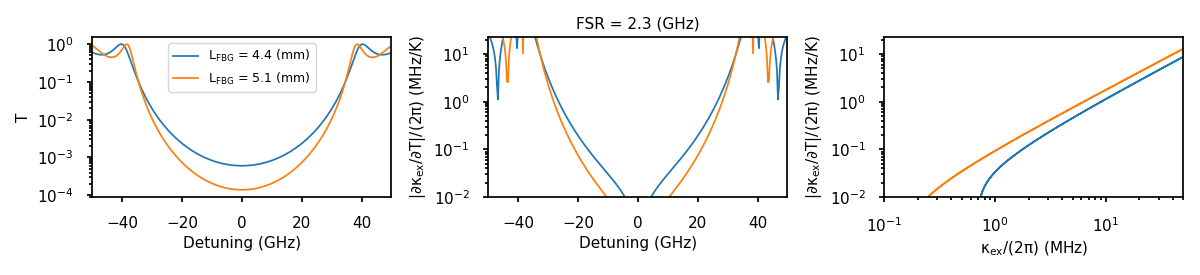
\includegraphics[width=1\linewidth]{fig/FBG_tuning.png}
% 	\caption{Cell number dependence of uniform FBG with $\delta n/n=4.3\times 10^{-4}$: $N_\mathrm{cell}=15000$, corresponding to FBG length of $4.4$ mm, respectively. Length between FBG regions, (left) $L_0=2$ mm, (middle) $5$ mm (right) $45$ mm, corresponding FSR of $0.5$, $2.3$ and $50$ GHz, respectively.}
%     \label{fig:fbgtuning}
% \end{figure}






\appendix

% \section{Model: Temperature and frequency dependence}
% To estimate the temperature of nanofiber by the cavity parameters, we consider a simple model: (1) the nanofiber is heated locally, leading to refractive index change $\delta n = \frac{\partial n}{\partial T}\delta T$ while the thermo elastic effect is negligible (one order magnitude smaller than thermo refractive one), (2) Fiber Bragg gratings add wavelength dependent phase shift due to the dispersion.  
% %Note that we can safely ignore the wavelength dependence of Silica refractive index $\delta n/\delta \lambda=1.55\times 10^{-5}/$ nm @ 852.3 nm by using the Sellmeier formular since we are interested in small range of the wavelength.
% Then, the round-trip phase shift in a cavity consists of propagation phase $\phi_\mathrm{nano}(T)$, $\phi_\mathrm{others}$ (\textit{nanofiber} regions and \textit{others} with the length of $L_\mathrm{nano}$ and $L_\mathrm{others}$, respectively) and dispersion of the FBGs $\phi_\mathrm{FBG}(\nu)$ as
% \begin{eqnarray}
%     \phi(\nu,T)&=&\phi_\mathrm{nano}(T)+\phi_\mathrm{others}+\phi_\mathrm{FBG}(\nu)\\
%     &=&\frac{4\pi \nu n_\mathrm{nano}(T)L_\mathrm{nano}}{c}+\frac{4\pi \nu  n_\mathrm{ot} L_\mathrm{others}}{c}
%     +\phi_\mathrm{FBG}(\nu)
% \end{eqnarray}
% where temperature of nanofiber region $T$.
% For typical scan of 40 GHz (or 0.1 nm), the refractive index change of Silica is $\delta n = 1.55 \times 10^{-6}$. Then, a $m$-th cavity resonance is written by 
% \begin{eqnarray}
%  \phi(\nu_m)=2\pi m \quad\rightarrow\quad
%     \nu_m &=& m\frac{c}{2 \mathcal{L}_\mathrm{cav}(\nu, T)}-\frac{c}{4\pi \mathcal{L}_\mathrm{cav}(\nu, T)}\phi_\mathrm{FBG}(\nu)\\
% \mathrm{where}\quad    \mathcal{L}_\mathrm{cav}(T)  &=&n_\mathrm{nano}(T)L_\mathrm{nano}+n_\mathrm{ot} L_\mathrm{others}
% \end{eqnarray}
% where optical path length $\mathcal{L}_\mathrm{cav}$. 
% The free spectral range is given by
% \begin{eqnarray}
%     \Delta_m\equiv\nu_m-\nu_{m-1}=
%     \frac{c}{2\mathcal{L}_\mathrm{
% cav}(\nu, T)}-\frac{c}{4\pi\mathcal{L}}\left(\phi_\mathrm{FBG}(\nu_m)-\phi_\mathrm{FBG}(\nu_{m-1})\right).
% \end{eqnarray}
% %is composed of a nanofiber and the rest of the sections, called, ``others''.
% The small change in optical path length due to the temperature change $\delta T$ is approximated by
% \begin{eqnarray}
%         \delta \mathcal{L}_\mathrm{cav}(T)\approx \frac{\partial n_\mathrm{nano}}{\partial T} L_\mathrm{nano}\delta T 
% \end{eqnarray}
% %Note that thermo elastic term is ignored since the thermo-refractive coefficient is one order of magnitude larger.
% Then, the change in a cavity resonance frequency $\delta \nu_m$ and the FSR $\delta \Delta_m$ (convenient observables) are given by 
% \begin{eqnarray}
%     \frac{\delta \nu_m}{\nu_m} &=&-\frac{L_\mathrm{nano}}{\mathcal{L}_\mathrm{cav}}\frac{\partial n_\mathrm{nano}}{\partial T}\delta T-\frac{c}{4\pi \mathcal{L}_\mathrm{cav}} \frac{\partial \phi_\mathrm{FBG}}{\partial \nu}\frac{\delta\nu}{\nu_m}
%     \label{eq:df}
% \\
%     \frac{\delta\Delta_m}{\Delta_m} &=&-\frac{L_\mathrm{nano}}{\mathcal{L}_\mathrm{cav}}\frac{\partial n_\mathrm{nano}}{\partial T}\delta T-\frac{c}{4\pi \mathcal{L}_\mathrm{cav}} \left(\frac{\partial \phi_\mathrm{FBG}}{\partial \nu}\Big|_{\nu_{m}}-\frac{\partial \phi_\mathrm{FBG}}{\partial \nu}\Big|_{\nu_{m-1}}
%     \right)\frac{\delta \nu}{\Delta_m}
% %    &\approx&-1.4\times 10^{-7} \delta T-1.0\times 10^{-6}\frac{\partial \phi_\mathrm{FBG}}{\partial \nu}\delta \nu
% \end{eqnarray}
% These relations suggest that cavity resonance shift $\delta\nu_m$ is practically suited for measuring the temperature due to the higher carrier frequency of the signal and better suppression of the FBG contribution ($\delta\nu/\nu_m$ vs $\delta\nu/\Delta_m$).  

% For instance, we take typical settings of $dn_\mathrm{nano}/dT\approx 10^{-5}, L_\mathrm{nano}=1$ mm, $\nu_m= 351.7
% $ THz (for Cs), and $ \mathcal{L}_\mathrm{cav}\sim n\cdot L_\mathrm{cav}$ with $n=1.454, L_\mathrm{cav}=5$ cm.
% Then, the frequency shift is evaluated to be 
% \begin{eqnarray}
%     \frac{\delta \nu_m}{\nu_m} 
%     \approx-1.4\times 10^{-7} \cdot\delta T-1.0\times 10^{-6}\cdot\frac{\partial \phi_\mathrm{FBG}}{\partial \nu}\delta \nu
%     \label{eq:df_num}
% \end{eqnarray}
% Note that the nonlinear temperature dependence can be incorporated by using $\frac{\partial n}{\partial T}=9.6\times 10^{-6}+7.7\times 10^{-9}\cdot (T-299~\mathrm{K})$.



% \subsection{Current scheme: Count cavity resonance numbers at the fixed frequency}
% ;The current procedure is to keep track of number of drifted cavity resonance from $1$-to-$N$ FSR at the fixed frequency ($\delta\nu=0$), allowing us to estimate the temperature drift without an effect from the FBG dispersion. 
% For instance,  by using Eq. (\ref{eq:df}), we obtain the case of 1 FSR shift $\Delta_m$ as,
% \begin{eqnarray}
%     \frac{\Delta_m}{\nu_m} =-\frac{L_\mathrm{nano}}{\mathcal{L}_\mathrm{cav}}\frac{\partial n_\mathrm{nano}}{\partial T}\delta T
%      \quad\rightarrow\quad
%     \delta T\approx\frac{\lambda}{2}\frac{1}{L_\mathrm{nano}\frac{\partial n_\mathrm{nano}}{\partial T}}\sim 40~\mathrm{K}
% \end{eqnarray}
% where $dn_\mathrm{nano}/dT\approx 10^{-5}, L_\mathrm{nano}=1$ mm.

% \subsection{Possibility of estimating temperature from cavity frequency change}
% The goal is to obtain a sensitivity to $\delta T=1$ K, corresponding to 
% $\frac{\delta \nu_m}{\nu_m}|_{\delta T}=-1.4\times 10^{-7}$ or $\delta \nu_m= 50$ MHz estimated by using Eq. (\ref{eq:df_num}).
% Ideally, we want to suppress the contribution from FBGs by 1/10-th of thermorefractive one as
% \begin{eqnarray}
% \delta\phi_\mathrm{FBG}=\frac{\partial \phi_\mathrm{FBG}}{\partial \nu}\delta\nu=1.4\times 10^{-2}\quad \mathrm{(rad)}
% \end{eqnarray}
% By using the estimated value of $\frac{\partial \phi_\mathrm{FBG}}{\partial}$ in Fig. \ref{fig:1dsim} (mimic a typical spectrum in the current system. See caption.) and assuming the symmetric cavity ($2\times \phi_\mathrm{FBG}$), we estimate the potential scanning range of frequency $\delta\nu$ as 
% \begin{eqnarray}
%     \mathrm{mid~gap:} &&\frac{\partial \phi_\mathrm{FBG}}{\partial \nu}\sim-0.037~\mathrm{rad/GHz~per~FBG}\quad\rightarrow\quad \delta \nu \sim 190~\mathrm{MHz}\\%\quad\leftrightarrow\quad \sim 8~\mathrm{K}\\
%     \mathrm{near~bandedge:} &&\frac{\partial \phi_\mathrm{FBG}}{\partial \nu}\sim-0.1~\mathrm{rad/GHz~per~FBG}\quad\rightarrow\quad \delta \nu \sim 70~\mathrm{MHz}
% \end{eqnarray}
% Practically, one can dither the heating beam intensity and extract the power-to-temperature coefficient once every ten seconds or more, set by the free-running stability of the cavity. 

% % \begin{figure}[!h]  
% %         \centering
% %         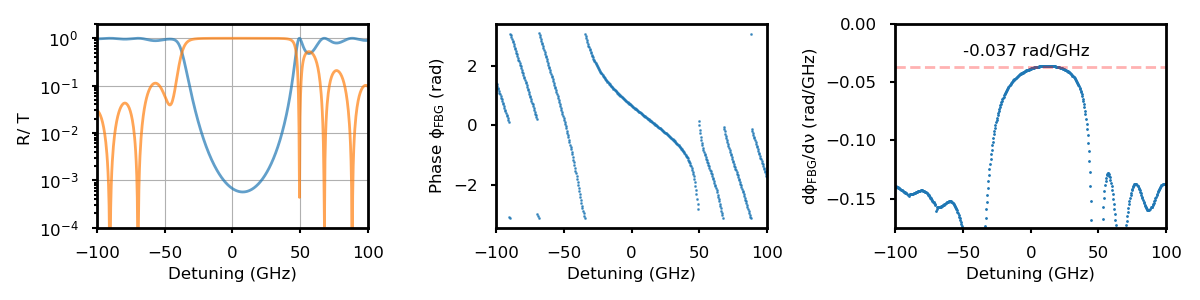
\includegraphics[width=1\linewidth]{fig/phase.png}
% % 	\caption{Transmission/Reflection spectra and phase shift of a single FBG, estimated by a 1D model including the spatial inhomogenity of refractive index modulation $\delta n$. The inhomogenity is hand-picked by using a gaussian envelope with $\sigma=5$ mm and peak $\delta n = 3.6\times 10^{-4}$, leading to the asymmetry of the transmission/reflection spectra with respect to detuning (typically observed in the current system). The most right plot shows $\frac{\partial \phi_\mathrm{FBG}}{\partial}\sim-0.037$ rad/GHz at the mid gap
% %  %and $\frac{\partial \phi_\mathrm{FBG}}{\partial}\sim-0.1$ rad/GHz near the bandedge.
% %  }
% %     \label{fig:1dsim}
% % \end{figure}



% %\textcolor{red}{[brief discussion about diameter dependence]}


\newpage

\section{Fiber Bragg grating}
The same summary as in Ref. \cite{note_temp}.
\label{app:1dmodel}
\subsection{1D model: uniformly alternate between $n$ and $n+\delta n$}
The FBG can be described by a 1D model with alternating two layers ($n_1, a_1)$ and $n_2, a_2)$. 
Analytical expressions of reflection and transmission coefficients are well know and convenient for later investigation as described in Ref. \cite{Bendickson1996}.
Here is a brief summary of key equations:
The transfer matrix of two layers ($n_1, a_1)$ and $n_2, a_2)$ is expressed by
\begin{eqnarray}
    M_{\mathrm{cell}}=\left(\begin{array}{cc}
1 / t^* & r / t \\
r^* / t^* & 1 / t
\end{array}\right)
\label{eq:tmat}
\end{eqnarray}
where $\phi_1=n_1 k a_1$, $\phi_2=n_2 k a_2$, and
\begin{eqnarray}
\frac{r}{t}  =\frac{i}{2}\left(\frac{-n_1}{n_2}+\frac{n_2}{n_1}\right) \sin \left(\phi_1\right) e^{-i\phi_2}, \quad
\frac{1}{t}  =\left(\cos \left(\phi_1\right)+\frac{i}{2}\left(\frac{n_1}{n_2}+\frac{n_2}{n_1}\right) \sin \left(\phi_1\right)\right) e^{i\phi_2}
\end{eqnarray}
The dispersion relation of an infinite 1D chain is given by using a unit cell length $a=a_1+a_2$ as
\begin{eqnarray}
%\mathrm{Tr}[M_\mathrm{cell}]&=&2\cos\beta a\\
    %\rightarrow
    \quad \cos (\beta a)&=&\cos \left(k n_1 a_1\right) \cos \left(k n_2 a_2\right)-\frac{1}{2}\left(\frac{n_1}{n_2}+\frac{n_2}{n_1}\right) \sin \left(k n_1 a_1\right) \sin \left(k n_2 a_2\right)
\end{eqnarray}
Then, $N$-periodic system is written by 
\begin{eqnarray}
    M_N=M_\mathrm{cell}^N = M_\mathrm{cell}\frac{\sin(N\beta a)}{\sin(\beta a)}-I\frac{\sin((N-1)\beta a)}{\sin(\beta a)}.
\end{eqnarray}
Thus, transmission, reflection coefficienta and phase are written by \cite{Bendickson1996}
\begin{eqnarray}
    \frac{r_N}{t_N}=\frac{r}{t}\frac{\sin(N\beta a)}{\sin(\beta a)}, \quad
    \frac{1}{t_N}=\frac{1}{t}\frac{\sin(N\beta a)}{\sin(\beta a)}-\frac{\sin((N-1)\beta a)}{\sin(\beta a)}
\end{eqnarray}
As shown in Fig. \ref{fig:dn_dep}, the larger bandgap ($\propto \delta n/n$) leads to the smaller $\partial \phi_\mathrm{FBG}/\partial T$.
%Note that the quarter-wave stack model is convenient to derive a compact form of $R/T$ and phase as shown in Ref. \cite{Bendickson1996}.
\begin{figure}[!h]  
        \centering
        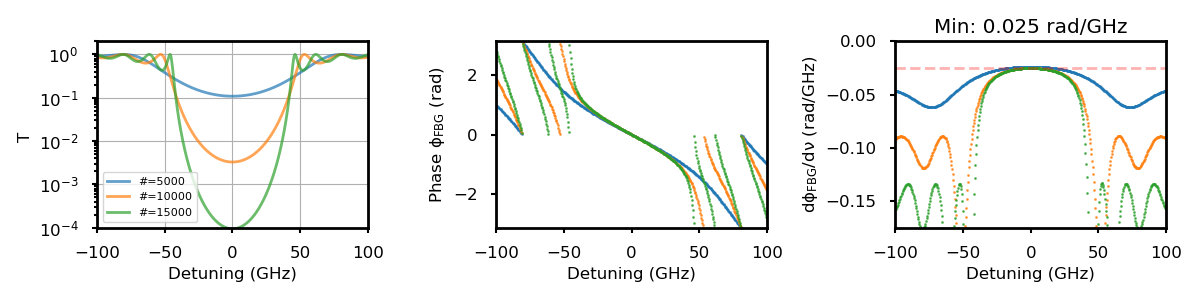
\includegraphics[width=1\linewidth]{fig/phase_21_20_17.png}
	\caption{Cell number dependence of uniform FBG with $\delta n/n=3.6\times 10^{-4}$: $N_\mathrm{cell}=5000, 10000, 15000$, corresponding to FBG length of $1.8$ mm, 3.6 mm and 5.3 mm, respectively. At the center of the bandgap, $d\phi_\mathrm{FBG}/d\nu = -0.025$ rad/GHz, independent of the cell number.}
    \label{fig:ncell_dep}
\end{figure}

\begin{figure}[!h]  
        \centering
        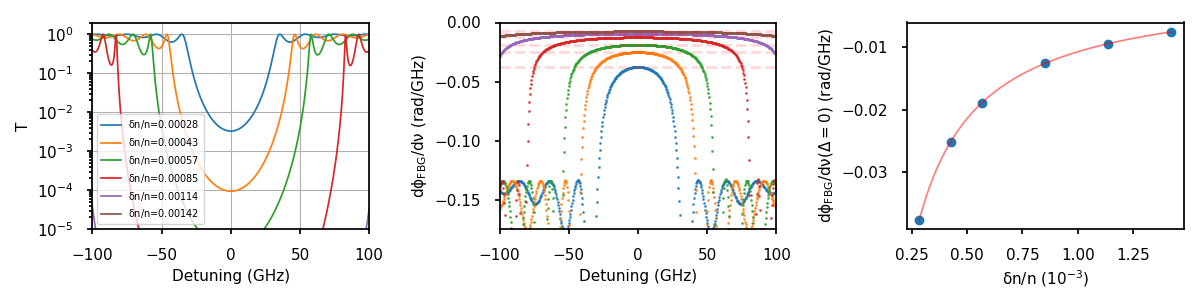
\includegraphics[width=1\linewidth]{fig/phase_22_17_23_25_26_24.png}
	\caption{Modulation $\delta n$ dependence with $N_\mathrm{cell}=15000$: As increasing the modulation amplitude $\delta n$, the band gap increases owing to $\Delta\nu_\mathrm{gap}/\nu=\delta n/n$. As a result, the slope the phase shift approaches to zero with a asymptotic form of $\frac{\partial \phi_\mathrm{FBG}}{\partial \nu} = \frac{A}{1+(\delta n/n)/B}$ where $A=-11.2(2.0), B=9.5(1.7)\times 10^{-7}$.}
    \label{fig:dn_dep}
\end{figure}
\vspace{-7mm}
\subsection{1D model: gaussian envelope of $\delta n$}
Using the transfer matrix of Eq. (\ref{eq:tmat}) with spatially dependent $\delta n$ (gaussian distribution with $\sigma = 5.9$ mm, N=17500), we numerically compute the $\tilde{M}_N = \prod_i^N M_\mathrm{cell}(\delta n_i)$ as shown in Fig. \ref{fig:fbgtuningGaussian}



\section{Strain-induced tuning}
The strain-induce wavelength shift is given by using the tenxile (axial) strain $\varepsilon$ as \cite{SkolianosThesis},
\begin{eqnarray}
    \frac{\delta \lambda}{\lambda} = \frac{\delta \Lambda}{\Lambda}+\frac{\delta n}{n}=\varepsilon+\frac{1}{n}\frac{\partial n}{\partial \varepsilon}\varepsilon\approx 0.78 \varepsilon\quad\mathrm{where}\quad \frac{1}{n}\frac{\partial n}{\partial \varepsilon}=-0.22
\end{eqnarray}
where the axial strain $\varepsilon$ is given by
\begin{eqnarray}
    \varepsilon=\frac{F}{EA}\quad\mathrm{where}\quad A=\frac{\pi d^2}{4}
\end{eqnarray}
and Young's modulus $E$ and diamter of the cylinder $d$. 
Thus, if forces are applied from both end of the fiber, strain in the middle is inversely proportional to diameter of the fiber, suggesting enhanced strain at the etched fiber by $\left(\frac{125}{30}\right)^2~14$ times.

\section{Surface-roughness to visibility: FBG inscription}
When the wavefront of the laser gets random phase perturbations $\phi(x)$ due to surface roughness, mutual coherence of the field at two points separated by $\Delta x$ is written by \cite{Leger1975}
\begin{eqnarray}
    \gamma(\Delta x)=\braket{e^{i(\phi(x)-\phi(x+\Delta x))}}
\end{eqnarray}
For a surface height $h(x)$ described by gaussian distribution with RMS roughness $\sigma$, we rewrite
\begin{eqnarray}
    \gamma(\Delta x)=\exp\left[-\left(\frac{4\pi}{\lambda}\right)^2\left(\sigma^2-C(\Delta x)\right)\right],\quad \mathrm{where}\quad C(\Delta x)=\braket{h(x)h(x+\Delta x)}
\end{eqnarray}
Beyond the surface correlation length $\xi$, resulting in $C(\Delta x)\rightarrow 0$, we simplify 
\begin{eqnarray}
    \gamma(\Delta x)=\exp\left[-\left(\frac{4\pi\sigma}{\lambda}\right)^2\right]\quad \mathrm{or}\quad \sigma = \frac{\lambda}{4\pi}\sqrt{-\mathrm{ln}V}
\end{eqnarray}
For example, the visibility of $V=0.5$ at $\lambda=213$ nm gives RMS fluctuation of 28 nm.

\bibliography{mybib} 

\end{document}
